\documentclass[12pt,a4paper]{article}

%\usepackage[left=1.5cm,right=1.5cm,top=1cm,bottom=2cm]{geometry}
\usepackage[in, plain]{fullpage}
\usepackage{array}
\usepackage{../../../pas-math}
\usepackage{../../../moncours}

\usepackage{multicol}
\usepackage{caption}


%\usepackage{pas-cours}
%-------------------------------------------------------------------------------
%          -Packages nécessaires pour écrire en Français et en UTF8-
%-------------------------------------------------------------------------------
\usepackage[utf8]{inputenc}
\usepackage[frenchb]{babel}
\usepackage[T1]{fontenc}
\usepackage{lmodern}
\usepackage{textcomp}



%-------------------------------------------------------------------------------

%-------------------------------------------------------------------------------
%                          -Outils de mise en forme-
%-------------------------------------------------------------------------------
\usepackage{hyperref}
\hypersetup{pdfstartview=XYZ}
%\usepackage{enumerate}
\usepackage{graphicx}
\usepackage{multicol}
\usepackage{tabularx}
\usepackage{multirow}


\usepackage{anysize} %%pour pouvoir mettre les marges qu'on veut
%\marginsize{2.5cm}{2.5cm}{2.5cm}{2.5cm}

\usepackage{indentfirst} %%pour que les premier paragraphes soient aussi indentés
\usepackage{verbatim}
\usepackage{enumitem}
\usepackage[usenames,dvipsnames,svgnames,table]{xcolor}

\usepackage{variations}

%-------------------------------------------------------------------------------


%-------------------------------------------------------------------------------
%                  -Nécessaires pour écrire des mathématiques-
%-------------------------------------------------------------------------------
\usepackage{amsfonts}
\usepackage{amssymb}
\usepackage{amsmath}
\usepackage{amsthm}
\usepackage{tikz}
\usepackage{xlop}
%-------------------------------------------------------------------------------



%-------------------------------------------------------------------------------


%-------------------------------------------------------------------------------
%                    - Mise en forme avancée
%-------------------------------------------------------------------------------

\usepackage{ifthen}
\usepackage{ifmtarg}


\newcommand{\ifTrue}[2]{\ifthenelse{\equal{#1}{true}}{#2}{$\qquad \qquad$}}

%-------------------------------------------------------------------------------

%-------------------------------------------------------------------------------
%                     -Mise en forme d'exercices-
%-------------------------------------------------------------------------------
%\newtheoremstyle{exostyle}
%{\topsep}% espace avant
%{\topsep}% espace apres
%{}% Police utilisee par le style de thm
%{}% Indentation (vide = aucune, \parindent = indentation paragraphe)
%{\bfseries}% Police du titre de thm
%{.}% Signe de ponctuation apres le titre du thm
%{ }% Espace apres le titre du thm (\newline = linebreak)
%{\thmname{#1}\thmnumber{ #2}\thmnote{. \normalfont{\textit{#3}}}}% composants du titre du thm : \thmname = nom du thm, \thmnumber = numéro du thm, \thmnote = sous-titre du thm

%\theoremstyle{exostyle}
%\newtheorem{exercice}{Exercice}
%
%\newenvironment{questions}{
%\begin{enumerate}[\hspace{12pt}\bfseries\itshape a.]}{\end{enumerate}
%} %mettre un 1 à la place du a si on veut des numéros au lieu de lettres pour les questions 
%-------------------------------------------------------------------------------

%-------------------------------------------------------------------------------
%                    - Mise en forme de tableaux -
%-------------------------------------------------------------------------------

\renewcommand{\arraystretch}{1.7}

\setlength{\tabcolsep}{1.2cm}

%-------------------------------------------------------------------------------



%-------------------------------------------------------------------------------
%                    - Racourcis d'écriture -
%-------------------------------------------------------------------------------

% Angles orientés (couples de vecteurs)
\newcommand{\aopp}[2]{(\vec{#1}, \vec{#2})} %Les deuc vecteurs sont positifs
\newcommand{\aopn}[2]{(\vec{#1}, -\vec{#2})} %Le second vecteur est négatif
\newcommand{\aonp}[2]{(-\vec{#1}, \vec{#2})} %Le premier vecteur est négatif
\newcommand{\aonn}[2]{(-\vec{#1}, -\vec{#2})} %Les deux vecteurs sont négatifs

%Ensembles mathématiques
\newcommand{\naturels}{\mathbb{N}} %Nombres naturels
\newcommand{\relatifs}{\mathbb{Z}} %Nombres relatifs
\newcommand{\rationnels}{\mathbb{Q}} %Nombres rationnels
\newcommand{\reels}{\mathbb{R}} %Nombres réels
\newcommand{\complexes}{\mathbb{C}} %Nombres complexes


%Intégration des parenthèses aux cosinus
\newcommand{\cosP}[1]{\cos\left(#1\right)}
\newcommand{\sinP}[1]{\sin\left(#1\right)}


%Probas stats
\newcommand{\stat}{statistique}
\newcommand{\stats}{statistiques}
%-------------------------------------------------------------------------------

%-------------------------------------------------------------------------------
%                    - Mise en page -
%-------------------------------------------------------------------------------

\newcommand{\twoCol}[1]{\begin{multicols}{2}#1\end{multicols}}


\setenumerate[1]{font=\bfseries,label=\textit{\alph*})}
\setenumerate[2]{font=\bfseries,label=\arabic*)}


%-------------------------------------------------------------------------------
%                    - Elements cours -
%-------------------------------------------------------------------------------




\date{}
\title{}


\begin{document}
	%\maketitle
	\chap[num=3, color=red]{Probabilités}{}
	
	\section{Vocabulaire}
	
	\subsection{Expérience, issue et probabilité}
	\begin{mydefs}
		\begin{itemize}
			\item En probabilités, on étudie les \kw{issues} d'une \kw{expérience aléatoire}.
			\item L'ensemble des issues de l'expérience forme \kw{l'univers}.
			\item On associe une \kw{probabilité $p_i$} à chaque issue.
			\item La \kw{somme des probabilités} de toutes les issues d'une expérience vaut \kw{1}.
			\item L'\kw{équiprobabilité} correspond au cas où toutes les issues de l'expérience ont la même probabilité de se produire.
		\end{itemize}
		
		
	\end{mydefs}
	
	\begin{myexs}
	\begin{enumerate}
		\item 	Soit ($u_n$) la suite arithmétique de terme initial $u_0 = 1,5$ et de raison $r = -7$.
		
		Le terme de rang $n$ est $u_n = 1,5 + n \times (-7)$ c'est à dire $u_n=1,5 - 7n$.
		
		On a ainsi : 
		\begin{itemize}
			\item $u_4 = 1,5 - 7 \times 4 = -26,5$
			\item $u_{100} = 1,5 - 7 \times 100 = -698,5$
		\end{itemize}
		
		\item Soit ($u_n$) la suite arithmétique de terme initial $u_1 = 14$ et de raison $r = 1,3$.
		
		Le terme de rang $n$ est $u_n = 14 + (n-1) \times 1,3$; c'est à dire $u_n = 12,7 + 1,3n$.

		On a ainsi : 
		\begin{itemize}
			\item $u_4 = 12,7 + 1,3 \times 4 = 17,9$;
			\item $u_{100} = 12,7 + 1,3 \times 100 = 142,7$.
		\end{itemize}
	\end{enumerate}

	
	
\end{myexs}
	
	\subsection{\'Evénements}
	
	\begin{mydefs}
		\begin{itemize}
			\item Un \kw{événement} A regroupe une partie des issues d'une expérience.
			\item La probabilité d'un événement A est $p(A)$.
			\item $\bar{A}$ est l'événement \kw{contraire} de A (voir figure \ref{fig:contraire}), on a $\bar{A}$ est $p(\bar{A}) = 1 - p(A)$.
			\item L'intersection de deux événements $A \cap B$ est l'ensemble des issues qui réalisent A \kw{ou} B (au moins un des deux). (Dans la figure \ref{fig:union}, la partie hachurée dans les deux sens)
			\item L'union de deux événements $A \cup B$ est l'ensemble des issues qui réalisent à la fois A \kw{et} B. (Dans la figure \ref{fig:union}, toutes les parties hachurées)
			
		\end{itemize}
	\end{mydefs}
	
	
	\vspace*{1cm}
	\begin{multicols}{2}
		\begin{center}
			
			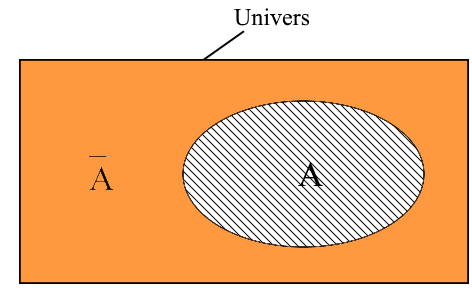
\includegraphics[scale=0.40]{./img/contraire}
			\captionof{figure}{Un événement et son contraire}
			\label{fig:contraire}
			
			
			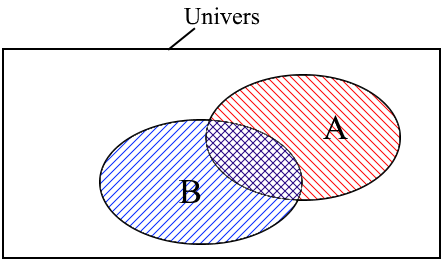
\includegraphics[scale=0.43]{./img/union_inter}
			\captionof{figure}{Union et intersection d'événements}
			\label{fig:union}
		\end{center}
		
		
<<<<<<< HEAD
	\end{multicols}	
	
	
	\begin{myex}
	La droite d'ajustement obtenue grâce au tableur passe par le point moyen $G$ dont nous avons calculé les coordonnées.
	\begin{center}
		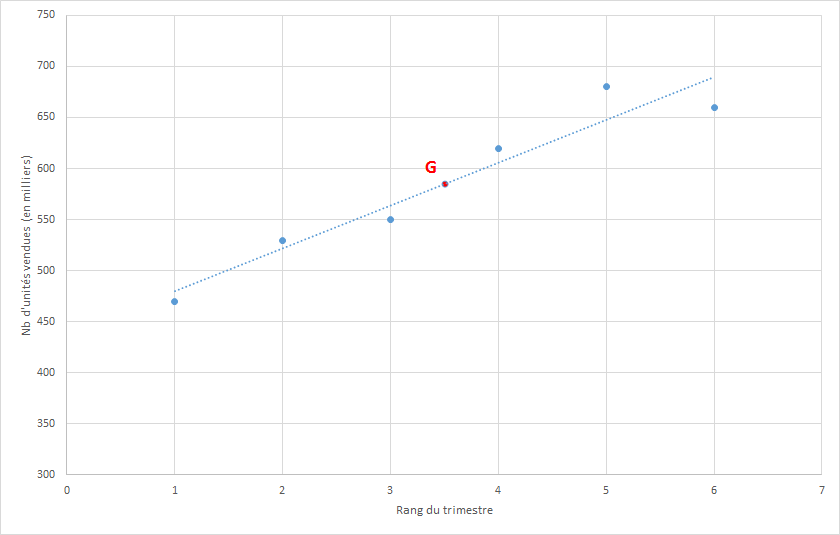
\includegraphics[scale =0.7]{./img/graph2}		
	\end{center}

\end{myex}
		
	\section{Calculs de probabilités}
	
	\subsection{Probabilité d'un événement}		
	
	\begin{myprops}
		\begin{itemize}
			\item La probabilité $p(A)$ d'un événement $A$ est la somme des propriétés des issues qui réalisent l'événement.
			\item En cas d'équiprobabilité on a : $p(A) = \dfrac{Nombre\;de\; cas\; favorables\; à\; A}{Nombre\; de\; cas\; possibles}$ .
		\end{itemize}
		
	\end{myprops}
	
	\begin{myex}
	Ici on considère la répartition des prix du gazole dans l'ensemble des 25 stations du département :
	
	\begin{center}
		\begin{tabular}{|@{\ }l@{\ } | @{\ }c@{\ } | @{\ }c@{\ } | @{\ }c@{\ } |@{\ }c@{\ } |@{\ }c@{\ } |@{\ }c@{\ }|@{\ }c@{\ }|@{\ }c@{\ }|@{\ }c@{\ }|@{\ }c@{\ }|}
			\hline
			Prix & 1,368 & 1,369 & 1,374 & 1,375 & \kw{1,377} & \kw{1,379} & 1,385 & 1,408 & 1,450 & 1,460 \\ \hline			
			Nb. de stations & 2 & 5 & 2 & 4 & 1 & 4 & 2 & 1 & 3 & 1 \\ \hline
		\end{tabular}
	\end{center}
	
	\kw{Moyenne} des prix des 25 stations : 
	\begin{center}
		$\bar{x} = \dfrac{1,368 \times 2 + 1,369 \times 5 + ... + 1,450 \times 3 + 1,460}{25} = 1,3884$
	\end{center}
	
	Le prix moyen observé pour ces 25 stations est 1,3884 €.	 
	
\end{myex}

	
	\begin{myex}
	On lance un dé à 6 faces non truqué. Puisque le de n'est pas truqué, nous sommes dans une situation d'équiprobabilité.
	On s'intéresse à l'événement A : <<le nombre obtenu est pair>>.	On a : 
	
	\begin{align*}
		p(A) &= p_2 + p_4 + p_6 \\
		&= \dfrac{1}{6} + \dfrac{1}{6} + \dfrac{1}{6} \\
		&= \dfrac{3}{6} \\
		&= 0,5
	\end{align*}
	
	Dans ce cas, la probabilité d'obtenir un résultat pair est de 0,5.
\end{myex}
	
	
	
	\subsection{Opérations sur les événements}
	
	
	
	
	
	
	
=======
		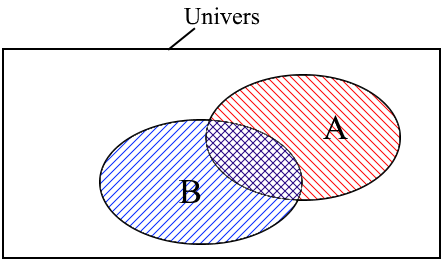
\includegraphics[scale=0.43]{./img/union_inter}
		\captionof{figure}{Union et intersection d'événements}
		\label{fig:union}
	\end{center}
 

\end{multicols}	


\begin{myex}
	La droite d'ajustement obtenue grâce au tableur passe par le point moyen $G$ dont nous avons calculé les coordonnées.
	\begin{center}
		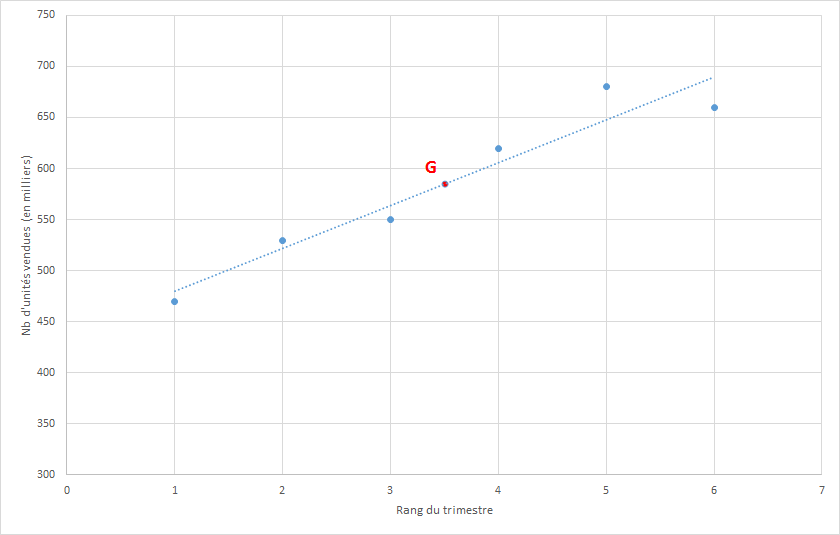
\includegraphics[scale =0.7]{./img/graph2}		
	\end{center}

\end{myex}
		
\section{Calculs de probabilités}

\subsection{Probabilité d'un événement}		

\begin{myprops}
	\begin{itemize}
		 \item La probabilité $p(A)$ d'un événement $A$ est la somme des probabilités des issues qui réalisent l'événement.
		 \item En cas d'équiprobabilité on a : $p(A) = \dfrac{Nombre\;de\; cas\; favorables\; à\; A}{Nombre\; de\; cas\; possibles}$ .
	\end{itemize}
	
\end{myprops}

\begin{myex}
	Ici on considère la répartition des prix du gazole dans l'ensemble des 25 stations du département :
	
	\begin{center}
		\begin{tabular}{|@{\ }l@{\ } | @{\ }c@{\ } | @{\ }c@{\ } | @{\ }c@{\ } |@{\ }c@{\ } |@{\ }c@{\ } |@{\ }c@{\ }|@{\ }c@{\ }|@{\ }c@{\ }|@{\ }c@{\ }|@{\ }c@{\ }|}
			\hline
			Prix & 1,368 & 1,369 & 1,374 & 1,375 & \kw{1,377} & \kw{1,379} & 1,385 & 1,408 & 1,450 & 1,460 \\ \hline			
			Nb. de stations & 2 & 5 & 2 & 4 & 1 & 4 & 2 & 1 & 3 & 1 \\ \hline
		\end{tabular}
	\end{center}
	
	\kw{Moyenne} des prix des 25 stations : 
	\begin{center}
		$\bar{x} = \dfrac{1,368 \times 2 + 1,369 \times 5 + ... + 1,450 \times 3 + 1,460}{25} = 1,3884$
	\end{center}
	
	Le prix moyen observé pour ces 25 stations est 1,3884 €.	 
	
\end{myex}


\begin{myex}
	On lance un dé à 6 faces non truqué. Puisque le de n'est pas truqué, nous sommes dans une situation d'équiprobabilité.
	On s'intéresse à l'événement A : <<le nombre obtenu est pair>>.	On a : 
	
	\begin{align*}
		p(A) &= p_2 + p_4 + p_6 \\
		&= \dfrac{1}{6} + \dfrac{1}{6} + \dfrac{1}{6} \\
		&= \dfrac{3}{6} \\
		&= 0,5
	\end{align*}
	
	Dans ce cas, la probabilité d'obtenir un résultat pair est de 0,5.
\end{myex}



\subsection{Utilisation d'un tableau de probabilités}


\begin{mymeth}
	On peut regrouper les différentes issues d'une expérience aléatoire dans un tableau.
	En transformant ce tableau en tableau de probabilités, on peut calculer plus facilement des combinaisons de deux événements.
\end{mymeth}



\begin{myex}
	Pour 500 personnes respirant des poussières pendant leur activité professionnelle on dispose des données suivantes :
	
	\begin{small}
		\begin{tabular}{@{\ }c@{\ }|@{\ }c@{\ }|@{\ }c@{\ }|@{\ }c@{\ }|}
			\cline{2-4}
			& Atteints de toux chronique & non atteins de toux chronique & Total \\ \hline
			\multicolumn{1}{|c|}{Fumeurs}     & 60                         & 140                           & 200   \\ \hline
			\multicolumn{1}{|c|}{Non fumeurs} & 40                         & 260                           & 300   \\ \hline
			\multicolumn{1}{|c|}{Total}       & 100                        & 400                           & 500   \\ \hline
		\end{tabular}
	\end{small}
	
	\vspace*{0.5cm}
	
	
	On prélève au hasard le dossier d'une personne parmi les 500.\\
	
	
	On note A l'événement << Le dossier est celui d'une personne atteinte de toux chronique>> et F <<Le dossier est celui d'un fumeur>>.\\
	
	Le tirage de  chaque dossier est équiprobable donc on peut utiliser les formule (nombre de cas favorables) divisé par (nombre de cas possibles).
	
	\begin{small}
		
		\renewcommand{\arraystretch}{2}
		\begin{tabular}{c|c|c|c|}
			\cline{2-4}
			& $A$                      & $\bar{A} $              & Total \\ \hline
			\multicolumn{1}{|c|}{$F$}         & $\dfrac{60}{500}=0,12$ & $\dfrac{140}{500}=0,28$ & 0.4   \\ \hline
			\multicolumn{1}{|c|}{$\bar{F}$} & $\dfrac{40}{500}=0,08$ & $\dfrac{260}{500}=0,52$ & 0.6   \\ \hline
			\multicolumn{1}{|c|}{Total}     & 0,2                    & 0,8                     & 1     \\ \hline
		\end{tabular}
	\end{small}
	
	$p(A \cup F) = 0,12 + 0,08 + 0,28 = 0,48.$
\end{myex}

>>>>>>> 7df5c2031162ed4727f320c52917a16f2eb611cb
	
	
	
\end{document}